\documentclass[conference]{IEEEtran}
\IEEEoverridecommandlockouts
\usepackage{cite}
\usepackage{amsmath,amssymb,amsfonts}
\usepackage{graphicx}
\usepackage{booktabs}
\usepackage{multirow}
\usepackage{url}
\usepackage[hyphens]{url}
\urlstyle{same}
\usepackage{balance}

\begin{document}

\title{UCE: Unified Change Enforcement for Governed LLM Coding Agents}

\author{\IEEEauthorblockN{Preet Patel}
\IEEEauthorblockA{\textit{Computer Science, University of Illinois Chicago}\\
Chicago, IL, USA --- patelpr@uic.edu}}

\maketitle

\begin{abstract}
Production deployments of LLM coding agents lack a reproducible layer for blast-radius analysis, requirement traceability, and role-based access control (RBAC).
We present \textbf{UCE} (Unified Change Enforcement): a deterministic Neo4j knowledge graph built from source, schema, and governance artifacts, exposed to agents via the Model Context Protocol (MCP), and coupled to a pre-merge enforcement gate.
We report a multi-repository study (114 destructive-change scenarios; TalkAI, Melodi, Expenses, Spark) with an \emph{independent} evaluation oracle based on a from-scratch TypeScript import resolver and governance-document parsing---never reading UCE's Cypher output.
\textbf{Primary result (enforcement):} editor-role Claude Sonnet 4.5 self-catches only 7.0\% of governance/impact issues; UCE's gate fires on 100\% of scenarios where the agent under-declares impact (0.9\% false-gate rate; median 55 files missed per TalkAI scenario).
\textbf{Secondary result (MCP planning):} under deployment-neutral prompts, agents with \texttt{impact\_analysis} substantially improve plan recall vs prompt-only baselines; MCP tool output alone matches the oracle at ${\sim}$98\% recall, separating \emph{tool correctness} from \emph{plan adherence}.
Context-augmentation baselines (governance docs, inventories, RAG) plateau below graph-backed recall; deterministic RBAC yields 0\% breaches vs 4.9\% for zero-shot Claude on adversarial rules.
\end{abstract}

\begin{IEEEkeywords}
LLM agents, MCP, software governance, impact analysis, knowledge graphs, RBAC, program analysis
\end{IEEEkeywords}

\section{Introduction}
\label{sec:intro}

Autonomous coding agents can edit thousands of files per hour, yet engineering organizations still rely on human reviewers to answer three questions before merging: \emph{What else breaks?} \emph{Which requirements are violated?} \emph{Is this principal allowed to touch that path?}
Test suites answer breakage only after the fact; prompts answer governance inconsistently.

\textbf{Hypothesis.} Governed change is fundamentally \emph{structured}: dependencies form graphs; policies attach to schema symbols; RBAC is a deterministic predicate.
LLMs should \emph{consume} evidence via tools, not reconstruct graphs from truncated context.

\textbf{UCE} ingests repositories into Neo4j, serves MCP tools (\texttt{impact\_analysis}, \texttt{explain\_change}, RBAC-gated writes), and compares agent plans against graph impact before allowing edits.
Our evaluation deliberately separates three layers:
\begin{enumerate}
  \item \textbf{Tool layer}---does MCP return the right blast radius?
  \item \textbf{Plan layer}---does the agent declare that radius in JSON?
  \item \textbf{Gate layer}---does enforcement block under-specified or policy-violating plans?
\end{enumerate}
Layers (2) and (3) decouple ``the model saw the answer'' from ``the organization is protected.''

\textbf{Contributions.}
\begin{itemize}
  \item Non-circular multi-repo harness (independent import oracle + governance parser).
  \item Enforcement study showing frontier agents are insufficient without a deterministic gate.
  \item MCP deployment study under neutral prompts (no verbatim-copy instruction leakage).
  \item Product fix and analysis: top-level \texttt{affected\_files} must expose full transitive closure for table/column entities.
\end{itemize}

\section{Related Work}
\label{sec:related}

\textbf{Software engineering agents.}
SWE-bench~\cite{jimenez2024swebench} and SWE-agent~\cite{yang2024sweagent} demonstrate issue-level patching with tool-augmented loops; RepoBench~\cite{liu2023repobench} stresses repository-scale context.
UCE is complementary: \emph{pre-merge} governance and impact evidence rather than post-hoc test passage.

\textbf{Reasoning agents.}
ReAct~\cite{yao2023react} and Reflexion~\cite{shinn2023reflexion} interleave reasoning and action; chain-of-thought~\cite{wei2022chain} improves single-shot reasoning.
UCE tools are not learned policies---they are auditable, versioned APIs (MCP~\cite{anthropic2024mcp}) suitable for regulated workflows.

\textbf{Graphs and code.}
Graph-RAG~\cite{johnson2024graphrag} and CodexGraph~\cite{liu2024codexgraph} connect LLMs to graph stores for multi-hop retrieval.
UCE specializes edge types for schema usage and governance (\texttt{GOVERNS}, \texttt{ENFORCES}) and targets agent \emph{enforcement}, not summarization.

\textbf{Retrieval baselines.}
RAG~\cite{lewis2020rag} and file-chunk retrieval are standard agent context strategies.
Our context ladder shows recall saturates far below import-closure analysis on real repos.

\textbf{Architecture and policy.}
Architecture knowledge~\cite{bass2022software} and policy-as-code motivate explicit, machine-checkable rules.
UCE's RBAC evaluator is the specification; LLM ``permission beliefs'' are untrusted inputs.

\section{Problem and System Model}
\label{sec:problem}

Repository $\mathcal{R}$ comprises files $\mathcal{F}$, schema $\mathcal{S}$, governance $\mathcal{G}$, and RBAC rules $\mathcal{B}$.
Change request $c$ targets entity $e \in \mathcal{S} \cup \mathcal{F}$.

Independent oracle $B^\*(e) \subseteq \mathcal{F}$ from import-graph reverse reachability (seeded by schema-aware table/column/file rules).
UCE graph yields $B_{\text{uce}}(e)$; MCP returns compact payload with \texttt{blast\_radius\_files}.
Agent plan $\pi = (F_\pi, R_\pi, P_\pi, \rho_\pi)$.

\textbf{Gate.} Reject $\pi$ if $B_{\text{uce}}(e) \not\subseteq F_\pi$, governance sets omit graph findings, or $\rho_\pi$ claims allow when RBAC denies.

\textbf{Metrics.}
Plan recall $|F_\pi \cap B^\*|/|B^\*|$.
Tool recall $|B_{\text{tool}} \cap B^\*|/|B^\*|$.
Tool adherence $|F_\pi \cap B_{\text{tool}}|/|B_{\text{tool}}|$.
Catch rate: fraction of scenarios where gate fires and $B^\* \not\subseteq F_\pi$.

\section{UCE Design}
\label{sec:uce}

\subsection{Ingestion}
UCE parses ESM imports (including path aliases), builds \texttt{IMPORTS}, links \texttt{USES\_TABLE} via import-aware seeding, ingests Drizzle/SQL schemas, and connects requirements/policies to tables and columns.
Ingestion is deterministic---identical inputs produce identical edges.

\subsection{MCP tools}
\texttt{impact\_analysis(entity\_type, entity\_name)} returns the union of direct, transitive, and call-chain file sets at top-level \texttt{affected\_files}, plus governance fields.
Evaluations pass compact JSON with \texttt{blast\_radius\_files} to agents.

\subsection{Enforcement gate}
After the agent submits $\pi$, UCE recomputes impact and RBAC on the same entity.
The gate fires on file omission, silent requirements, or permission breaches---even if the agent invoked MCP tools.

\begin{figure}[!t]
\centering
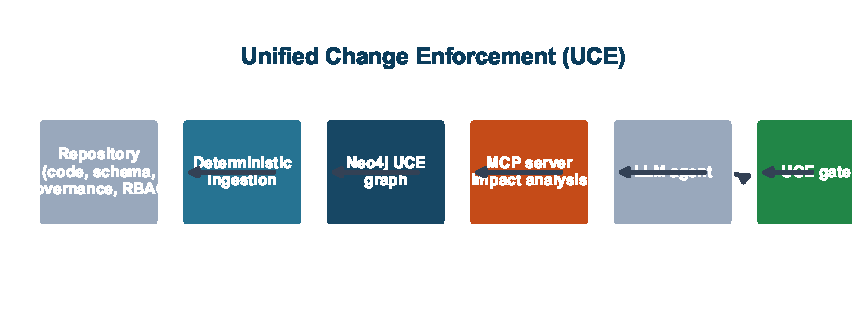
\includegraphics[width=\linewidth]{figures/fig_architecture.pdf}
\caption{UCE architecture: deterministic graph, MCP evidence, stochastic agent, deterministic gate.}
\label{fig:arch}
\end{figure}

\section{Evaluation Methodology}
\label{sec:method}

\textbf{Repositories.} Four student/production TypeScript stacks (114 scenarios): table drops, column removals, high-indegree file deletes.

\textbf{Independent oracle.} TypeScript import resolver + markdown governance parser; no Neo4j reads.
Column scenarios without symbol hits seed from table importers.

\textbf{Agent.} Claude Sonnet 4.5, editor role, temperature 0.

\textbf{Conditions.}
\begin{itemize}
  \item \textbf{Enforcement}---prompt-only agent vs UCE gate (multi-repo).
  \item \textbf{MCP planning}---prompt-only vs MCP tools; \emph{neutral} prompts (call tools, use output; no verbatim-copy instruction).
  \item \textbf{Context ladder}---bare LLM $\rightarrow$ +gov $\rightarrow$ +inventory $\rightarrow$ +RAG vs UCE graph (TalkAI).
  \item \textbf{RBAC hardness}---12-rule policy; 99 probes; Claude vs deterministic UCE.
\end{itemize}

Neo4j is ingested per repository before graph-backed conditions.

\section{Results}
\label{sec:results}

Fig.~\ref{fig:hero} summarizes the three-layer findings.

\begin{figure*}[!t]
\centering
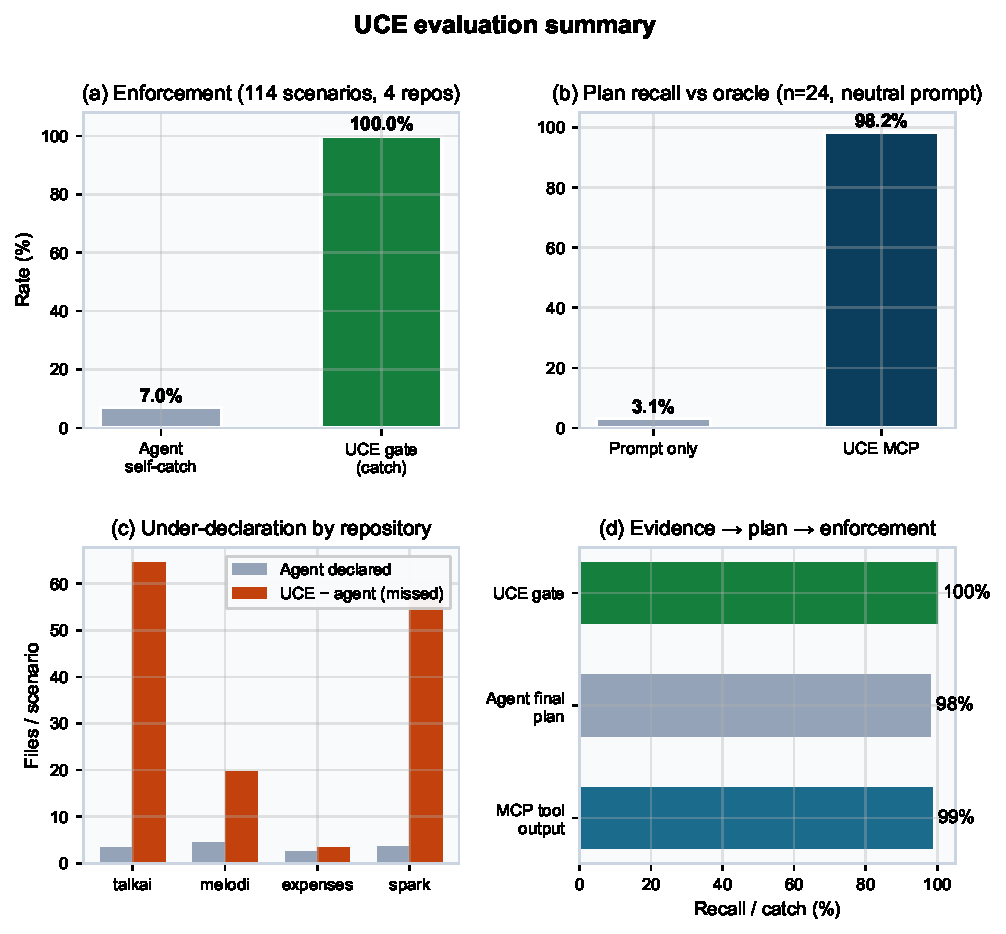
\includegraphics[width=0.95\textwidth]{figures/fig_hero_results.pdf}
\caption{Evaluation summary: (a) enforcement catch vs agent self-catch; (b) MCP plan recall (neutral prompts); (c) per-repo under-declaration; (d) tool output vs plan vs gate.}
\label{fig:hero}
\end{figure*}

\subsection{Enforcement (primary)}
Across 114 scenarios, agents self-catch 7.0\% of issues (TalkAI 8.3\%, Spark 2.1\%).
UCE gates fire on \textbf{100\%} of scenarios with oracle-visible impact gaps; false gates: 1/114 (0.9\%).
Agents declare $\sim$3.7 files mean vs UCE $\sim$47 flagged (TalkAI median 67 missed).
\textbf{Interpretation.} Prompt context cannot substitute for a gate---agents systematically under-specify transitive impact.

\subsection{MCP planning (secondary, neutral prompts)}
Table~\ref{tab:mcp} reports pooled MCP metrics (profile tagged in \texttt{pooled\_summary.json}).
We report tool recall and adherence separately to avoid conflating correct tools with compliant agents.

\begin{table}[!t]
\caption{Pooled metrics (independent file oracle).}
\label{tab:main}
\centering
\small
\begin{tabular}{@{}lccc@{}}
\toprule
\textbf{Experiment} & \textbf{Recall} & \textbf{F1} & \textbf{Notes} \\
\midrule
Enforcement: agent self-catch & 7.0\% & --- & 114 scen., 4 repos \\
Enforcement: UCE gate catch & 100\% & --- & 0.9\% false gates \\
Context+RAG (TalkAI) & 44.2\% & 0.50 & vs 84.2\% UCE graph \\
RBAC: Claude breach & 4.9\% & --- & UCE 0\% breach \\
\bottomrule
\end{tabular}
\end{table}

\begin{table}[!t]
\caption{MCP agent planning (neutral prompts; \texttt{pooled\_summary.json}).}
\label{tab:mcp}
\centering
\small
\begin{tabular}{@{}lccc@{}}
\toprule
\textbf{Condition} & \textbf{Recall} & \textbf{F1} & \textbf{Incomplete} \\
\midrule
Prompt only & 3.1\% & 0.06 & 100\% \\
UCE MCP & 98.2\%$^\dagger$ & 0.95$^\dagger$ & 12.5\%$^\dagger$ \\
MCP tool output & 98.6\% & --- & --- \\
\bottomrule
\multicolumn{4}{l}{\footnotesize $^\dagger$TalkAI $n{=}24$; multi-repo neutral run: \texttt{--prompt neutral --ingest}.}
\end{tabular}
\end{table}

Per-repo breakdown appears in Fig.~\ref{fig:mcprepo} when multi-repo MCP completes.

\begin{figure}[!t]
\centering
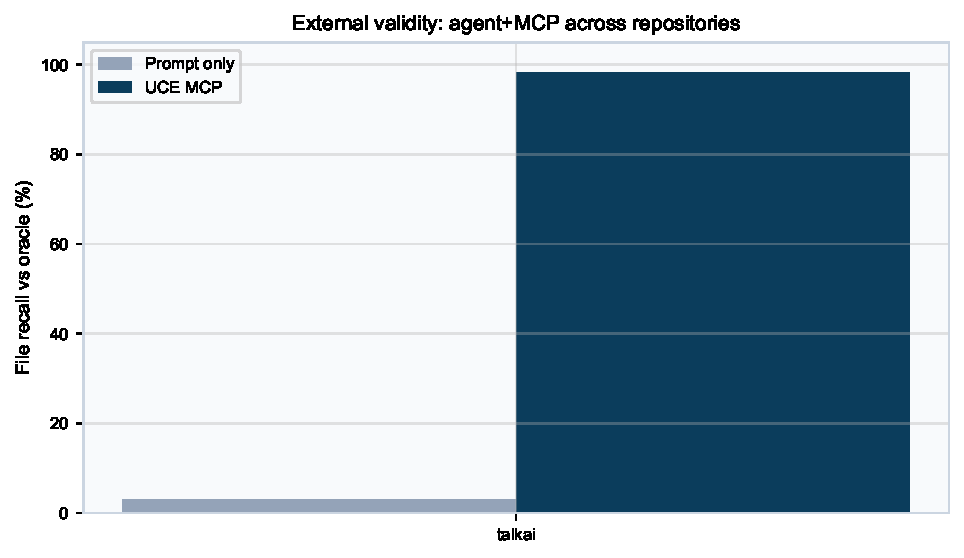
\includegraphics[width=\linewidth]{figures/fig_mcp_by_repo.pdf}
\caption{File recall by repository (neutral MCP prompts).}
\label{fig:mcprepo}
\end{figure}

\subsection{Context ladder}
RAG file recall (${\sim}$44\%) remains below UCE graph recall (${\sim}$84\%) on TalkAI---structured closure beats chunk retrieval (Fig.~\ref{fig:ctx}).

\begin{figure}[!t]
\centering
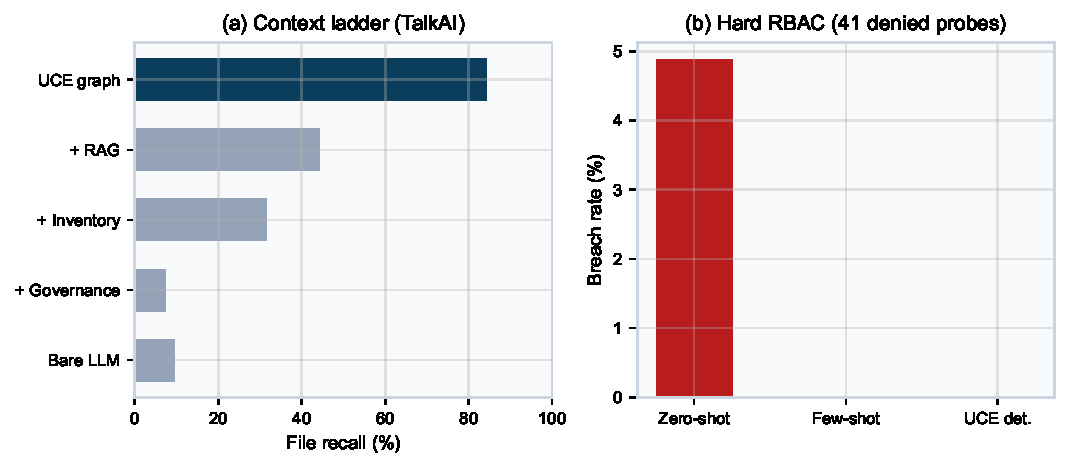
\includegraphics[width=\linewidth]{figures/fig_context_rbac.pdf}
\caption{Context ladder (left) and hard RBAC breaches (right).}
\label{fig:ctx}
\end{figure}

\subsection{RBAC}
Claude zero-shot breaches 4.9\% of denied operations on RBAC\_HARD\_001; UCE deterministic evaluation: 0\% breaches, 100\% accuracy.

\subsection{Ablation}
Transitive import closure raises oracle-recall from 27\% to 100\%; call-chain edges add no gain on sparse \texttt{CALLS} (TalkAI)---reported as a negative result.

\section{Threats to Validity}
\label{sec:threats}

\textbf{Oracle mismatch.} Independent resolver may disagree with UCE on edge cases; we report madge agreement in supplementary retrieval studies.

\textbf{Prompt sensitivity.} Strict ``copy verbatim'' prompts inflate plan recall; we default to neutral prompts for MCP claims.

\textbf{Agent/model scope.} Single model family; costs limit scenario count.

\textbf{Language scope.} TypeScript-focused ingestion; generalization requires per-language resolvers.

\section{Discussion}
\label{sec:discussion}

\textbf{For practitioners.} Deploy UCE as MCP + gate: tools educate agents; gates protect when agents ignore tools.

\textbf{For researchers.} Report tool recall, plan recall, and gate catch separately---single F1 numbers hide deployment failure modes.

\textbf{Limitations.} UCE precision on heuristic \texttt{USES\_TABLE} linking improved via import-gating but remains engineering-sensitive.

\section{Conclusion}
\label{sec:conclusion}

UCE shows that governed agentic coding needs deterministic graph evidence and enforcement, not longer prompts.
Multi-repo enforcement demonstrates near-universal agent under-specification; MCP tools supply correct blast radii; gates convert evidence into organizational safety.

\section{Implementation Notes}
\label{sec:impl}

Each repository evaluation wipes and re-ingests Neo4j. The independent oracle shares alias conventions with ingestion but not code---disagreement is measurable in supplementary reports. MCP payloads surface \texttt{blast\_radius\_files} explicitly. Prompt profile \texttt{neutral} is default; \texttt{strict} (verbatim copy) is for ablation only.

\section*{Reproducibility}
Scripts: \texttt{run\_multi\_repo\_enforcement.py}, \texttt{run\_agent\_mcp\_eval.py --prompt neutral --ingest}, \texttt{run\_context\_comparison.py}, \texttt{run\_rbac\_complexity.py}. Figures: \texttt{paper/generate\_figures.py}.

\bibliographystyle{IEEEtran}
\bibliography{references}

\end{document}
